\documentclass{article}
\usepackage{main}
\usepackage{amsmath}

\begin{document}

\title{Supplementary material}
\maketitle
\tableofcontents
\newpage
\renewcommand{\thefigure}{S\arabic{figure}}
\setcounter{figure}{0}

\section{Information Criteria for Local Clocks}
Clockor2 uses the AIC, AICc, and BIC to compare local clock models. Here we begin by giving the formula for each. Each criterion depends on the number of samples ($n$), number of inferred parameters ($k=3$ per clock), and the likelihood of the model fit ($\hat{L}$). We capitalise upon the assumption of independent sampling in root-to-tip regression to factorise the likelihood and calculate information criteria for local clock models.

\begin{equation}
    \textnormal{BIC} = k\ln{n} - 2\ln{\hat{L}}
\end{equation}
\begin{equation}
    \textnormal{AIC} = 2k - 2\ln{\hat{L}}
\end{equation}
\begin{equation}
    \textnormal{AICc} = \frac{2k^2+2k}{n-k-1} + k\ln{n} - 2\ln{\hat{L}}
\end{equation}

We begin with the example of two local clocks before generalising to an arbitrary number of clocks. Consider a tree with $n$ tips and 2 local clocks. Each local clock is comprised of a group of tips $g_1$ and $g_2$, such that $ \|g_1\| + \|g_2\| = n $

The log-likelihood, containing the product of probability densities for each data point, can then be factored into the sum of log likelihoods for each local clock:
\begin{equation}
    \ln{\hat{L}} = \sum_{i=1}^{2} \ln{\hat{L}_{g_{i}}}
\end{equation}

The number of inferred parameters is also $k = 6 = 2\cdot3$ (intercept, variance, slope).

For example, we can then write the BIC as:
\begin{equation}
    \textnormal{BIC} = 6\ln{n} - 2\sum_{i=1}^{2} \ln{\hat{L}_{g_{i}}}
\end{equation}

Generalising to the case where we have $c$ local clocks, the BIC then becomes:
\begin{equation}
    \textnormal{BIC} = (3c)\ln{n} - 2\sum_{i=1}^{c} \ln{\hat{L}_{g_{i}}}
\end{equation}

\section{Efficiency of the Clock Search Algorithm}
We briefly provide reasoning for why the clock search algorithm operates in polynomial time.
Consider a tree with $n$ tips, and a clock search that searches for a maximum of $c$ clocks each of a minimum size $s$, ensuring that $cs \le n$.

Given there are $n$ tips, there are then $2(n-1)$ internal nodes from which a clock can descend, and for a given number of clocks $1,...,c$, there are $p$ internal nodes such that a local clock can descend from each and induce a group with more than $s$ tips ($\|g\| \ge s$). $p$ depends on the topology of the tree (denoted as $t$) as well as the number of clocks ($c$) and minimum group size ($s$), so we now write $p(t,c,s)$ with $1 \le p(t,c,s) \le n$.

The number of possible combinations of nodes that can be chosen to fit $c$ local clocks, each of at least size $s$ is then:
\begin{equation}
    \binom{p(t,c,s)}{c} = \frac{p(t,c,s)!}{c!(p(t,c,s)-c)!}
\end{equation}

That is, the clock search is polynomial in $p(t,c,s)$. $p(t,c,s)$ is related to $n$ by the topology of the particular tree being searched, so we assert for generality that the clock search is polynomial in $n$. $p(t,c,s) = n$ when $c = s = n$.

Finally, the clock search searches for $1,...,c$ clocks, completing in a number of steps equal to:
\begin{equation}
    \sum_{1}^{c} \binom{p(t,c,s)}{i}
\end{equation}

The number of steps can be reduced by reducing the maximum number of clocks searched for ($c$) and/or increasing the minimum group size ($s$).

As noted above, tree topology also affects $p(t,c,s)$, in turn affecting the number of steps taken in the clock search. We expect topology to have the smallest effect on efficiency compared to the other parameters ($s$, $t$), and it is usually expected to be beyond the control of the researcher anyway. For completeness, we note that a perfectly balanced tree requires the most steps for the algorithm to complete while a completely imbalanced, ladder tree would require the least.

\section{\textcolor{red}{Clock-search Simulation Study}}
\subsubsection*{Methods}
We conducted a simulation study to test the accuracy of the clock-search algorithm. \textcolor{red}{We first simulated a core set of 100 rooted trees with 250 tips under the Birth-Death process using TreeSim \citep{stadler_2011_simulating}. We added noise to root to tip distances by randomly adding or substracting an amount from 0 to half the original branch length. That is:
\begin{equation*}
    b^{\prime}= b + U[-0.5b,~0.5b],~\textnormal{where $b$ is the original branch length}
\end{equation*}
For each tree, we added a local clock descending from a randomly selected node such that it would contain between 50 and 150 tips. We then simulated a 5-fold rate increase along the descending branch alone, and again throughout the descending clade, yielding a set of 200 trees. These scenarios are characterised in Fig 1 B,D (main text) respectively and referred to as the stem and stem+clade cases from hereon. In each case there 100 trees with background and foreground rates of $1\times10^{-3}$ and $5\times10^{-3}$ \textit{subs/site/time}, as in Fig 1. In addition, we retained the original 100 trees without adding rate acceleration to use this as a test case for false positives where there are no local clocks. We refer to this as the global case  from hereon. For each of the 300 trees, we applied the clock search algorithm with a minimum group size of 50 tips and a maximum number of of 2-4 clocks. In the stem and stem+clade cases, a maximum of 2 clocks tests for baseline accuracy with the search parameters matching reality.} Searches with a maximum of 3-4 clocks test for over-sensitivity in the algorithm where the maximum number of clocks is inflated. All clock-search tests use the BIC.

\subsection*{Results and guidelines}
\begin{figure}[H]
\centering
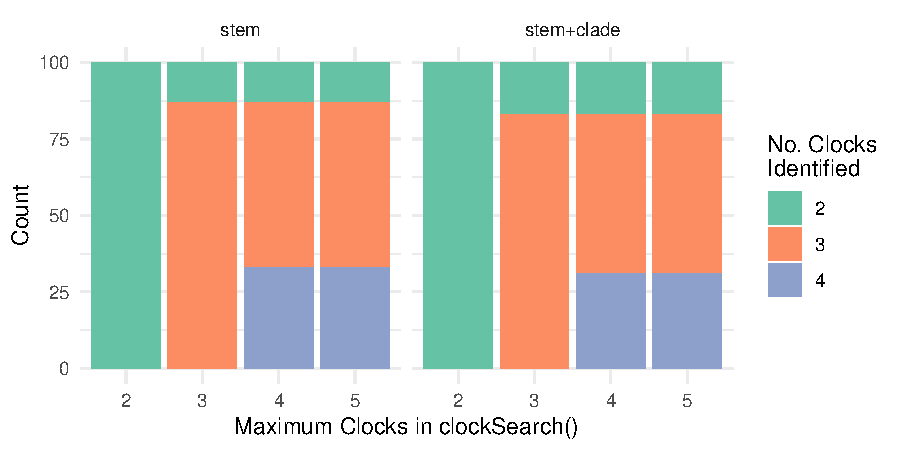
\includegraphics[width = \linewidth]{inferredClocks.pdf}
\caption{\textcolor{red}{Confusion matrices comparing the number of inferred clocks against the maximum number of clocks allowed by each search. In the global panel, the true value is 1 global clock, which none of the searches selected.  The stem and stem+clade panels refer to either a rate increase along only the stem of a clade, or with the rate increase throughout clade, with a true value of 2 local clocks. Accuracy decreases as the maximum number of clocks allowed by the clock-search algorithm increases. The colour and number in each tile reflect the number of analyses out of 100 in each column selecting the corresponding number of clocks.}}
\label{fig:simStudy}
\end{figure}

\textcolor{red}{In the global case, searches never recovered the true value of 1 global clock. All searches instead selected 2 local clocks where the maximum allowed number of clocks was 2. Subsequent searches also tended to select the maximum possible when 3 and 4 local clocks were allowed. This prompted our first guideline of not using the clock search unless there is a biological hypothesis for the existence of local clocks.}

\textcolor{red}{For the stem only and stem+clade cases, the clock-search algorithm correctly identified 2 local clocks in all cases where the maximum number of allowed clocks was 2 (Fig. \ref{fig:simStudy}). However, when the algorithm was allowed to search for configurations with 3-4 clocks, only 16 and 14 analyses correctly recovered 2 clocks.}
Although we used the BIC, the most conservative information metric used in Clockor2, the clock-search algorithm is clearly still highly prone to over-fitting. This is because a higher number of clocks allows for tighter clusters of points in the RTT regression to be found, which are favoured over a lower number of clocks.

\begin{figure}[H]
\centering
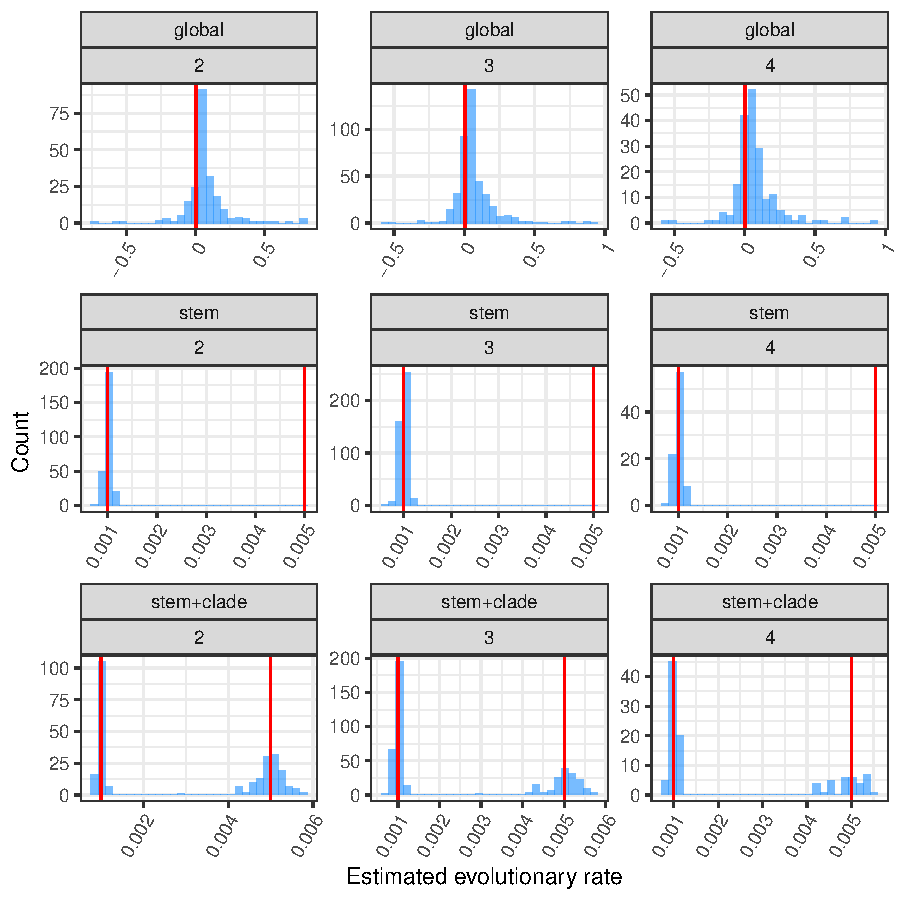
\includegraphics[width = 0.8\linewidth]{clockError.pdf}
\caption{\textcolor{red}{Histograms of the evolutionary rate for each inferred local clock in the simulation study. Plot labels refer to the simulation study case (global, stem, or stem+rate), and the maximum number of clocks allowed by each clock search (2, 3, or 4). Red vertical lines mark the true values for evolutionary rates in each local clock. These are $1\times10^{-3}$ and $5\times10^{-3}$ \textit{subs/site/time} for the stem and stem+clade cases, and $1\times10^{-3}$ and \textit{subs/site/time} for the global case. Overall, inferred evolutionary rates are congruent with the true underlying values.}}
\label{fig:clockError}
\end{figure}

\textcolor{red}{In support of this explanation, we also found that where clock searches for the stem and stem+clade cases inflated the number of clocks, the inferred rate of evolution remained congruent with the true value Fig \ref{fig:clockError}. In the stem case, this corresponds to inferred rates clustering around $1\times10^{-3}$ \textit{subs/site/time} since rate acceleration only occurs on the branch separating clocks, such that each have the same rate. In the stem+clade case this corresponds to estimated rates clustering around $1\times10^{-3}$ and $5\times10^{-3}$ \textit{subs/site/time}. In the global case, we recovered a similar pattern but noted that the discrepancy between the true and inferred evolutionary rates to be slightly higher. Estimates were congruent with true values overall, but there were 13 inferred clades with inferred evolutionary rates above $1$ \textit{subs/site/time}. In these cases, such configurations can be easily discarded by eye. Taken together, these results support the user following guidelines:\newline
1) Do not use the clock search where there is no biological hypothesis to support it. \newline
2) Do not conduct a search with more clocks in the search than are hypothesised.}

\begin{figure}[H]
\centering
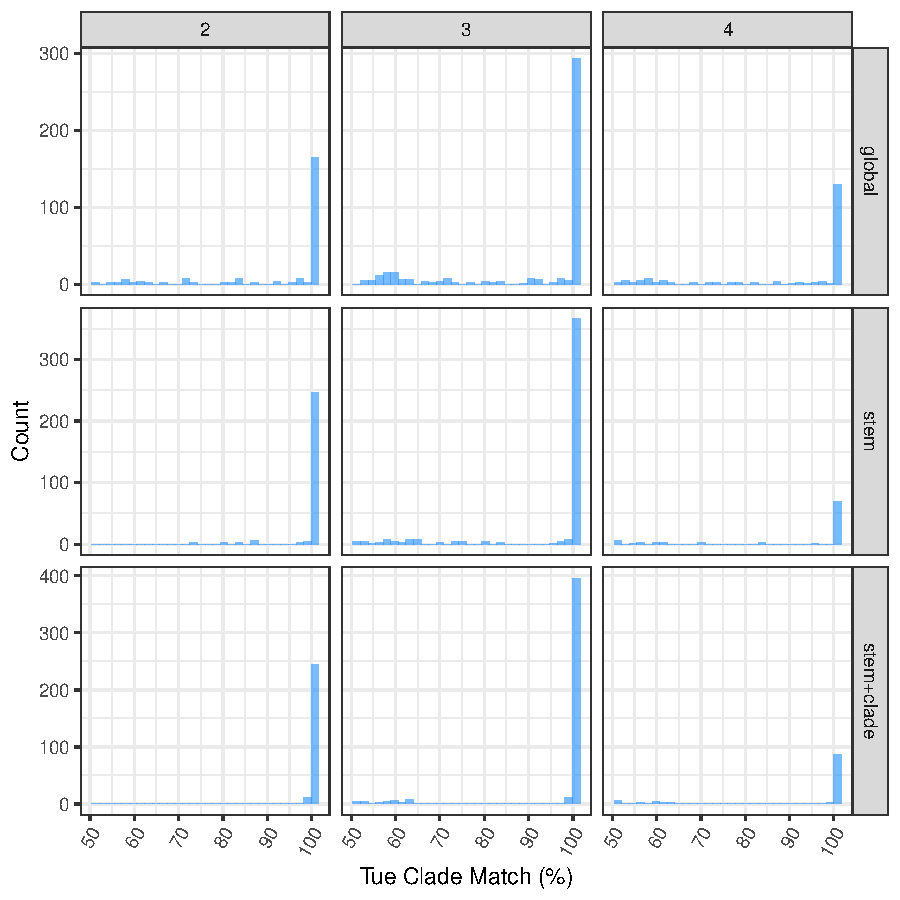
\includegraphics[width = 0.7\linewidth]{cladeMatch.pdf}
\caption{\textcolor{red}{Histograms of the percentage match for each inferred local clock in the simulation study to the most similar true local clock group. Values of 100\% indicate that all tips in a local clock co-occur in the true underlying local clock. Plot labels refer to the simulation study case (global, stem, or stem+rate), and the maximum number of clocks allowed by each clock search (2, 3, or 4). The majority of inferred local clocks fell within one of true local clocks across each simulation condition.}}
\label{fig:cladeMatch}
\end{figure}

\textcolor{red}{Last, we found that tip groups from inferred local clocks corresponded to the true underlying local clocks in the stem and stem+clade cases (Fig \ref{fig:cladeMatch}). This also provides strong evidence that the cause of over-parameterisition in the local clock search comes from sub-clustering tips within true local clocks, rather than conflating tips into arbitrary groups.}

To this end, we again emphasise that the clock-search algorithm is only intended to be used as a tool testing a number of clocks up to and including the hypothesised number, \emph{but never more}. It should also never be used to blindly search for local clocks in the absence of a biological hypothesis. The \href{https://clockor2.github.io/clockor2/}{Clockor2 how-to documents} (\url{https://clockor2.github.io/clockor2/}) provide example of over-fitting using the clock search function when applied to various empirical datasets \citep{porter2023evolutionary,dudas_mers-cov_2018}.
\newpage

\section{Best Fitting Root Targeting Residual Mean Squared}
When searching for the best fitting root, for each proposed root there is the question of where to place the root between the two descending branches to maximise temporal signal. In Clockor2, this point is selected by maximising $R^2$, or minimising the residual mean squared. For the residual mean square, there is an analytical solution for this point that we derive here.

The following is an independent derivation by LAF of the algorithm implemented in Tempest and derived by Luiz Max Carvalho.

First, define the following:
\begin{enumerate}

    \item $L$ is the sum of basal branch lengths leading to the left and right root-child.
    \item {$d_i$}, The set of root-to-tip distances where all basal branch length ($L$) is shifted to the branch leading to the right root-child.
    \item {$t_i$}, The sampling times associated with each $d_i$
    \item {$c_i$}, An indicator variable indicating whether a tip descending from the left or right root-child. $c_i = -1$ if descending from the left child, and $c_i = 1$ if descending from the right.
    \item $x$ is the portion of total branch length $L$ that we add to $d_i$ descending from the left root-child and subtract from $d_i$ descending from the right root-child
\end{enumerate}

Now, to capture the different to root-to-tip distances that come with shifting the root position, we define:
\begin{equation}
\begin{aligned}
    d^{\prime}_i = d_{i} + c_{i}x
\end{aligned}
\end{equation}

And we seek to minimise with respect to $x$ the Residual Mean Square:
\begin{equation}
    \textnormal{RSM}(x) = \frac{1}{n-2}\sum_{i}(\hat{d^{\prime}_i} - d^{\prime}_i)^2
\end{equation}

Which is equivalent to minimising the Residual Sum of Squares(RSS)
\begin{equation}
\begin{aligned}
    \textnormal{RSS}(x) = \sum_{i}(\hat{d^{\prime}_i} - d^{\prime}_i)^2 \\
    = S_{d^{\prime}d^{\prime}} - S_{td^{\prime}}^2S_{tt}^{-1}
\end{aligned}
\end{equation}

\begin{equation}
\begin{aligned}
        \textnormal{Where } S_{d^{\prime}d^{\prime}} = \sum_{i}(\bar{d^{\prime}} - d^{\prime}_i)^2,
        S_{tt}= \sum_{i}(\bar{t} - t_i)^2, \textnormal{ and } 
        S_{d^{\prime}t} = \sum_{i}(\bar{d^{\prime}}-d_i)(\bar{t}-t_i)
\end{aligned}
\end{equation}

Subbing $d^{\prime}_i = d_{i} + c_{i}x$ into each of $S_{d^{\prime}d^{\prime}}$, $S_{tt}$, and $S_{d^{\prime}t}$, we come to:
\begin{equation}
\begin{aligned}
    \textnormal{RSS}(x) = S_{dd} - 2xS_{dc} + x^{2}S_{cc} - S_{tt}^{-1}(S_{dt} - 2xS_{dt}S_{tc} + x^{2}S_{tc}^{2})
\end{aligned}
\end{equation}


Observe that RSS($x$) is quadratic in $x$, and that $ \textnormal{RSS} \ge 0$, so there must be a global minimum we can solve for.

We therefore solve:

\begin{equation}
\begin{aligned}
    &\frac{d}{dx}\textnormal{RSS}(x) = 0 \\
    &\implies  -2S_{dc} + 2xS_{cc} + 2S_{td}S_{tc}S_{tt}^{-1} - 2xS_{tc}^{2}S_{tt}^{-1} = 0 \\
    &\implies x = \frac{S_{dc}-S_{ty}S_{tc}S_{tt}^{-1}}{S_{cc}-S_{tc}^2S_{tt}^{-1}}
\end{aligned}
\end{equation}

Finally, it may be that $x > L$. For this reason, Clockor2 internally relies on $\alpha = \frac{x}{L}$, the proportion of $L$ assigned to the left branch under the best fitting root. Then, we take the following as the solution:

\begin{equation}
\begin{aligned}
    \alpha = \max \left \{ \min \left \{ \frac{S_{dc}-S_{td}S_{tc}S_{tt}^{-1}}{L(S_{cc}-S_{tc}^2S_{tt}^{-1})} \right \}, 1), 0  \right \} 
\end{aligned}
\end{equation}

\newpage
\bibliography{clockor2}

\end{document}